The KNN algorithm was implemented by interpreting each feature, or in this case
every document, as a dimension and feature values corresponds to the term
occurrence frequencies. The distance function used in the algorithm was the
euclidean distance function. It could have been interesting to test other
function as well but this was not prioritized and the euclidean distance function
was chosen since it seemed to be the most straight forward method to calculate
the distance. Calculations
of the nearest neighbours were implemented in a non deterministic way. This
because of that a point $x$ in a plane may have neighbours with the property
that they have equal distances to $x$. If this is the case a nearest neighbour
is chosen at random. Several choices for $k$ were tested in different runs of
the algorithm to find the best $k$ for the classification. The algorithm was
implemented to be able to classify both different classes (music , software,
etc.) and sentimental classification (positive, negative). Figure
\ref{fig:KNNplot} shows the misclassification done by the algorithm for both
different $k$ and different sizes of the feature sets. The plot was generated
with training set size 2000 and test set size 100 for unigrams. Note that the
result might look different for other training set sizes. We used the best $k$
from this plot.
\begin{figure}[h!]
\centering
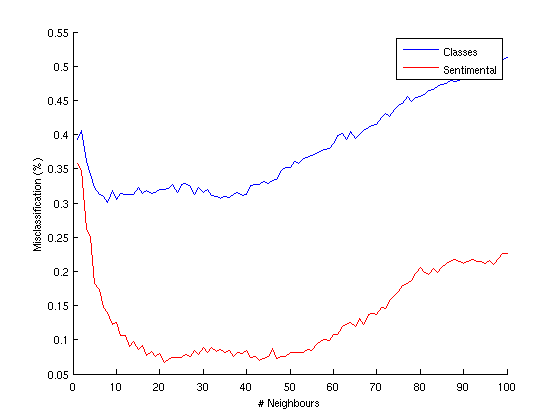
\includegraphics[scale=0.6]{../Plottar/knn_2000words_testdata100_unigram}
\caption{Plot showing results from the KNN classifier}
\label{fig:KNNplot}
\end{figure}\\
Figure \ref{fig:KNNplot} shows that KNN has best performance with parameter $K = 20$ for sentimental and $K = 10$ for classes.

